\section{Appendix}\label{sec:appendices}
% -------------------------------------- 
\subsection{Datasets}\label{appx:datasets}
\import{okapi}{datasets.tex}

\subsection{Relation to Algorithmic Fairness}\label{appx:fairness}
\import{okapi}{fairness.tex}

\subsection{Extended Results}\label{appx:ext_results}

We present in Table~\ref{tab:ext_iw_pm_results} an extended version of the results for the iWildCam
and PovertyMap datasets, relative to those found in Table~\ref{tab:iw_pm_results} in the main text.
%
This table includes additional results with the ResNet backbones per \citet{SagWeiLeeGaoetal22} --
justifying our decision to adopt a ConvNext backbone for our main set of image-dataset results --
as well as those for an 'offline' version of Okapi (Okapi (offline)) where the matches are
generated prior to training using features of the respective \ac{ERM} baseline for each dataset. 
%
Since the target encoder is necessitated by the need for online match-retrieval, only a single
encoder is involved in Okapi (offline); in binary cases, the algorithm is then identical to the one
proposed by \citet{RomInsShaQua22} with the exception that consistency is still enforced via
distance in encoding space rather than with a JSD loss on the predictive distributions which fails
to generalise to regression tasks such as PovertyMap.

\import{okapi}{ext_results.tex}

\subsection{Implementation details}\label{appx:implementation}
\import{okapi}{implementation.tex}

\subsection{Additional Matching Examples}\label{appx:additional_matches}

\begin{figure}[ht!]
  \centering
  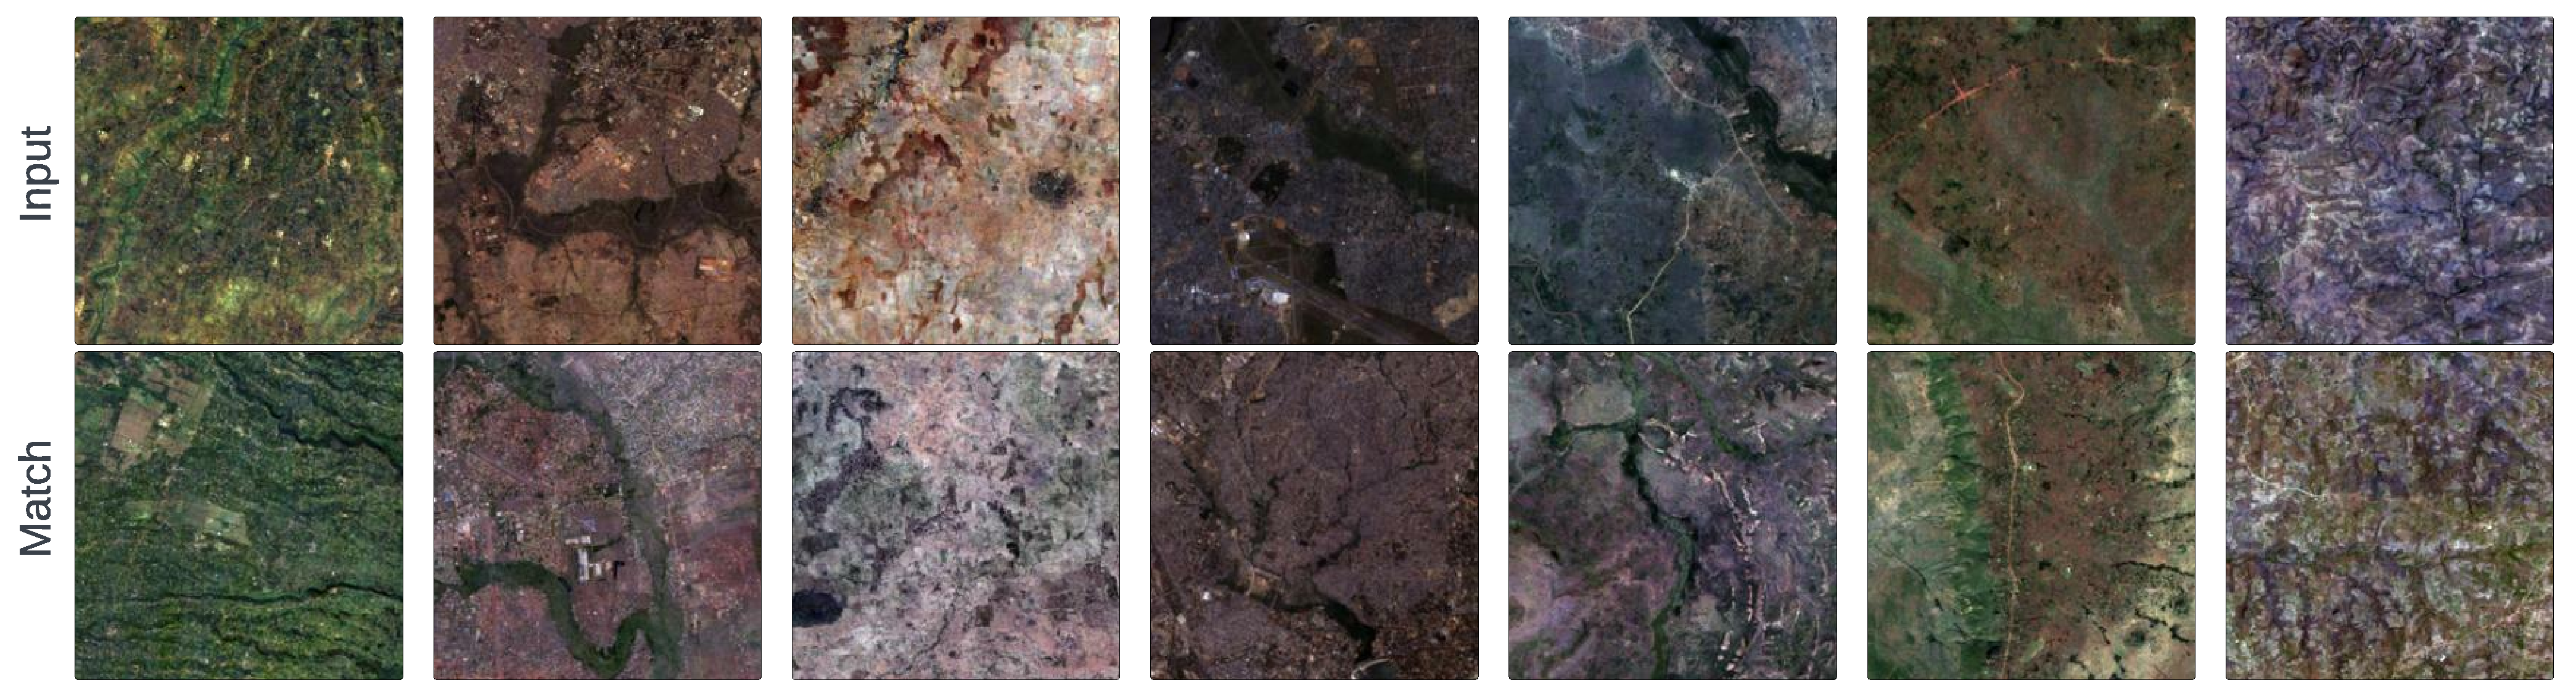
\includegraphics[width=1.\textwidth]{figures/matches_examples_pm.pdf}
  \caption{
      Examples of input (labelled) images and their 1-NN matched (unlabelled) images retrieved
      using \CNN{} from the PovertyMap-WILDS dataset.
      %
      Here, we match images from the labelled-train set to images from the \ac{OOD}-validation set,
      taking advantage the fact that their domains are disjoint.
  %
  }
 \end{figure}
 
\subsection{Ablations}\label{appx:ablations}

\import{okapi}{tables/pm_ablations.tex}

 We supplement the ablation experiment on the use of calipers featured in the main text with
 additional experiments concerning effect of the number of nearest neighbours ($k$), the relative
 importance of the two (fixed and std) calipers, and the feasibility of using the online encoder as
 the query-generator instead of the target encoder.
 %
 The results of these experiments are tabulated in \ref{tab:ablations} with the key takeaways
 being: \begin{enumerate} 
     \item The number of neighbours used for computing the consistency loss
         has little impact -- according to the given level of precision -- on the performance of Okapi
        along all axes.
     \item While disabling the calipers altogether considerably harmed performance, using only the
         std. caliper allows us to recover the performance of the complete algorithm,
         (\texttt{Okapi (k=5)}), whereas the same is not true for the fixed caliper which, while
         aiding performance compared to the no-caliper baseline, falls short of that benchmark.
         %
         A caveat attached to these conclusions, however, is that the selected values for $\xi$ are
         likely suboptimal in the online setting, given that they were optimised for the static
         setting: with improved selection of $\xi$, either by learning it jointly with the model's
         parameters (using, for instance, the perturbed maximum method \citep{berthet2020learning}
         to overcome the non-differentiability of the $k$-NN and thresholding operations), in an
         amortised fashion, or optimising it on a per-iteration basis.
         %
    \item While less appealing from a conceptual standpoint, due to the mismatch between the
        networks used to generate the queries and keys, from an empirical standpoint it is
        perfectly feasible to use the online encoder to generate the queries for statistical
        matching instead the target encoder while experiencing minimal degradation in performance.
        %
        This is particularly relevant when one wishes to perform the matching in only one direction
        (e.g.\ \( \gD_l \to \gD_l \)) due to the reduction in redundant encoding, with each encoder
        only encoding its respective subset of the data (e.g. $f_\theta$ only encodes samples from
        $\gD_l$, \( f_\theta^\prime \) only encodes samples from \( \gD_u \)
\end{enumerate}


\subsection{Pseudocode}\label{appx:pseudocode}
%
\import{okapi/pseudocode/}{calipernn.tex}
\import{okapi/pseudocode/}{ol.tex}
%
\noindent We give PyTorch-style \citep{paszke2019pytorch} pseudocode for the \CNN{}
(described in~\ref{subsec:matching}) and online-learning (described in~\ref{subsec:ol}) algorithms
in Algorithm~\ref{alg:calipernn_pc} and Algorithm~\ref{alg:ol_pc}, respectively.
In both cases, we restrict the pseudocode to the special case of binary domains --
 practically achieved by using the labelled/unlabelled as a proxy for domain -- 
for ease of illustration.
The \CNN{} algorithm can be generalised freely to multiclass cases by considering pairwise
interactions between the propensity scores for each domain for applying the calipers and by
computing the pairwise inequalities between $\mbf{s}_q$ and $\mbf{s}_k$ (giving the connectivity
matrix \( (\mbf{s}_q \cdot \mbf{1}^T) \neq (\mbf{1} \cdot \mbf{s}_k^T) \), where $\mbf{1}$ denotes the
ones vector of the same shape as its multiplicand and mediates broadcasting) for enforcing the
cross-domain constraint.
 
\subsection{Matching for PACS dataset}\label{appx:pacs_matching}

In this section, we discuss results from initial experiments on the PACS
dataset~\citep{li2017deeper} (using features extracted for a pre-trained CLIP
\citep{radford2021learning} visual encoder) showing how the temperature scaling can be used to
smooth the propensity score distribution to better control how many sample are discarded during
matching. 
% 
There are 1,670 \emph{photo}, 2,048 \emph{art painting}, 2,344 \emph{cartoon}, and 3,929
\emph{sketch} in the dataset. Here will evaluate the results of matching across the two domains
\emph{photo} and \emph{art painting} as well as across \emph{photo} and \emph{sketch}.
% 
In Fig.~\ref{fig:pacs_ps_pa} and Fig.~\ref{fig:pacs_ps_ps} we compare the shape of the estimated
propensity score with its scaled version using a temperature value of 10. 
%
As we can see, in the case of a distribution with extremely heavy tails (photo, sketch), the effect
of smoothing the distribution is that when a fixed caliper is applied most of the samples are
retained. 
%
On the other hand, when the initial distribution is smoother, a temperature of 10 is extreme,
having the effect of transforming the bimodal distribution to a unimodal one.
% 
Additionally, we tabulate in Table~\ref{tab:pacs_nsamples} the number of matched pairs retrieved
when matching across the two domains photo and sketch; here we can see that by increasing the
temperature we smooth the estimated propensity score distribution and thereby retain more samples.
%
Similarly, we can retrieve more pairs by reducing the fixed caliper threshold. 
%
We also analyse the case of matching across the two domains photo and art painting. Using a fixed
caliper defined defined by a threshold \( t_f = 0.1 \) and no temperature scaling (i.e.\ $\tau=1$)
the algorithm retrieves 1,142 pairs matching in the direction photo $\to$ art and 1,501 in the
direction art $\to$ photo. 
% 

In Fig.~\ref{fig:match_pairs_pa} and Fig.~\ref{fig:match_pairs_ps} we show examples of matching
pairs found using our \CNN{} algorithm. Although the features were not fine-tuned on PACS, we can
see a few examples of intraclass matching. For the photo-art painting application we can see
preservation in colour and background; while in the photo-sketch case shape and pose.

\begin{figure}[ht!]
     \centering
     \begin{subfigure}[b]{0.49\textwidth}
         \centering
         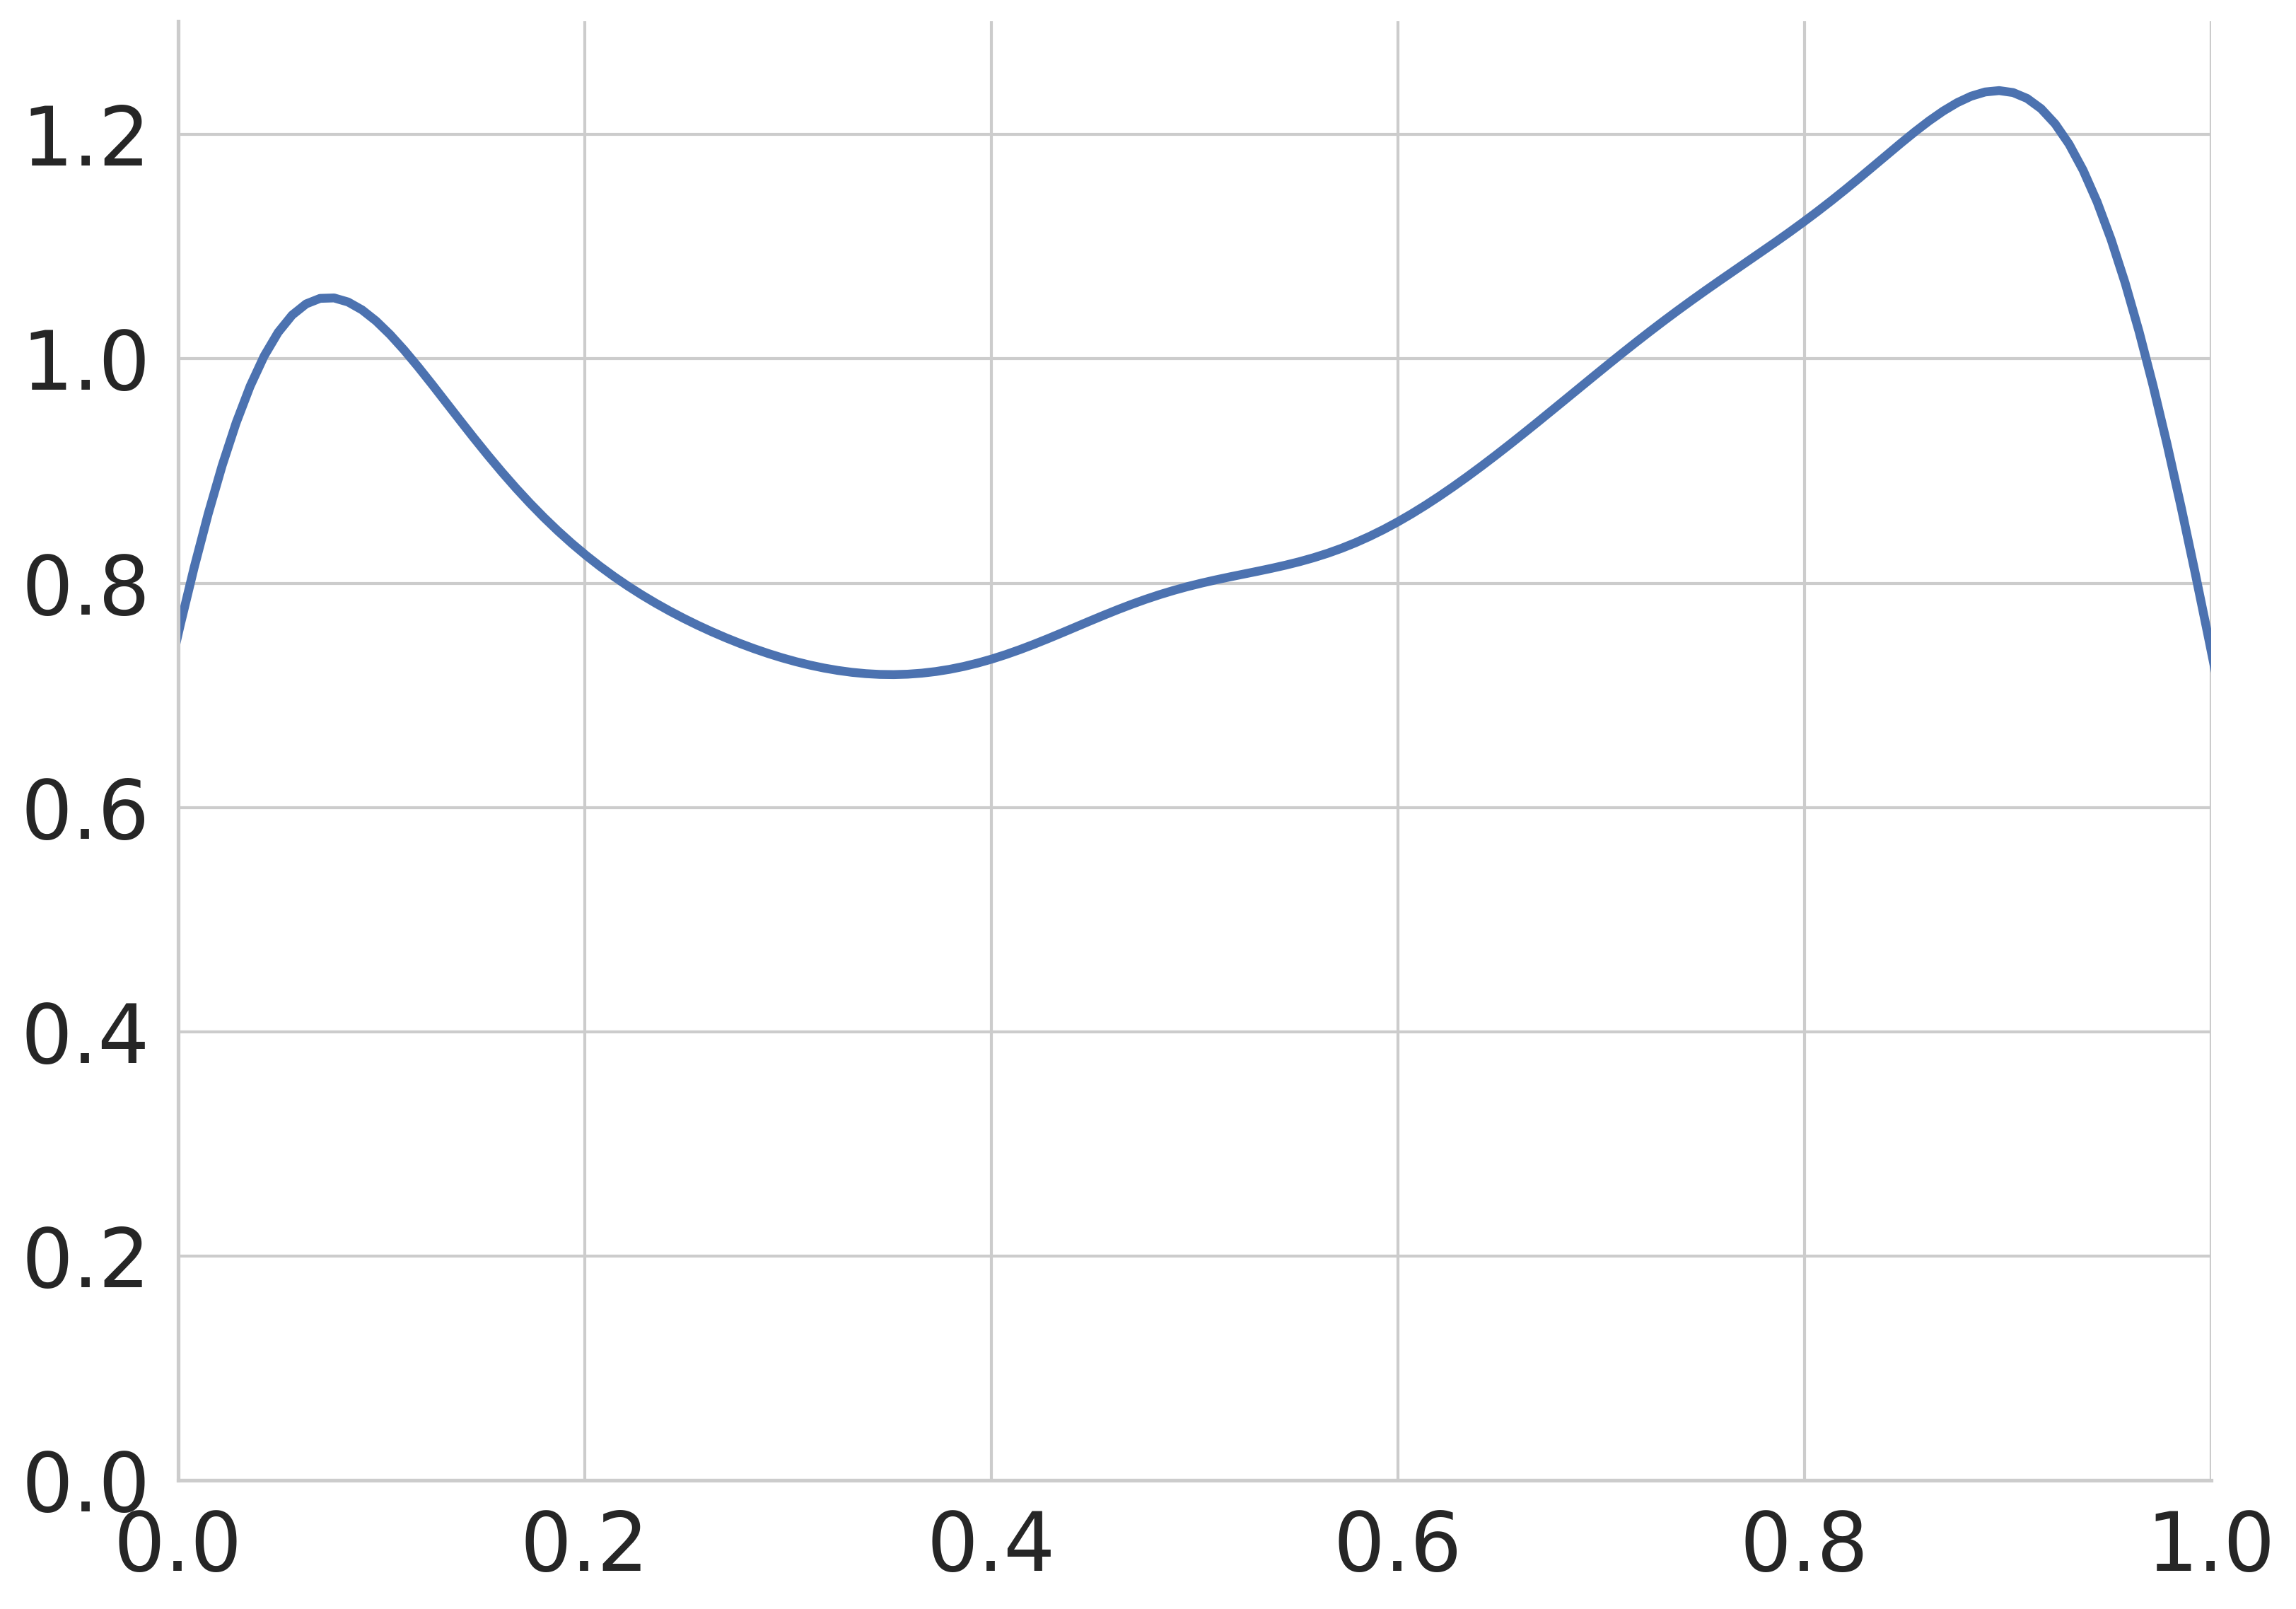
\includegraphics[scale=0.2]{figures/ps_photo_artpainting_temp1.png}
         \caption{No temperature scaling ($\tau=1$).}
     \end{subfigure}
     \hfill
     \begin{subfigure}[b]{0.49\textwidth}
         \centering
         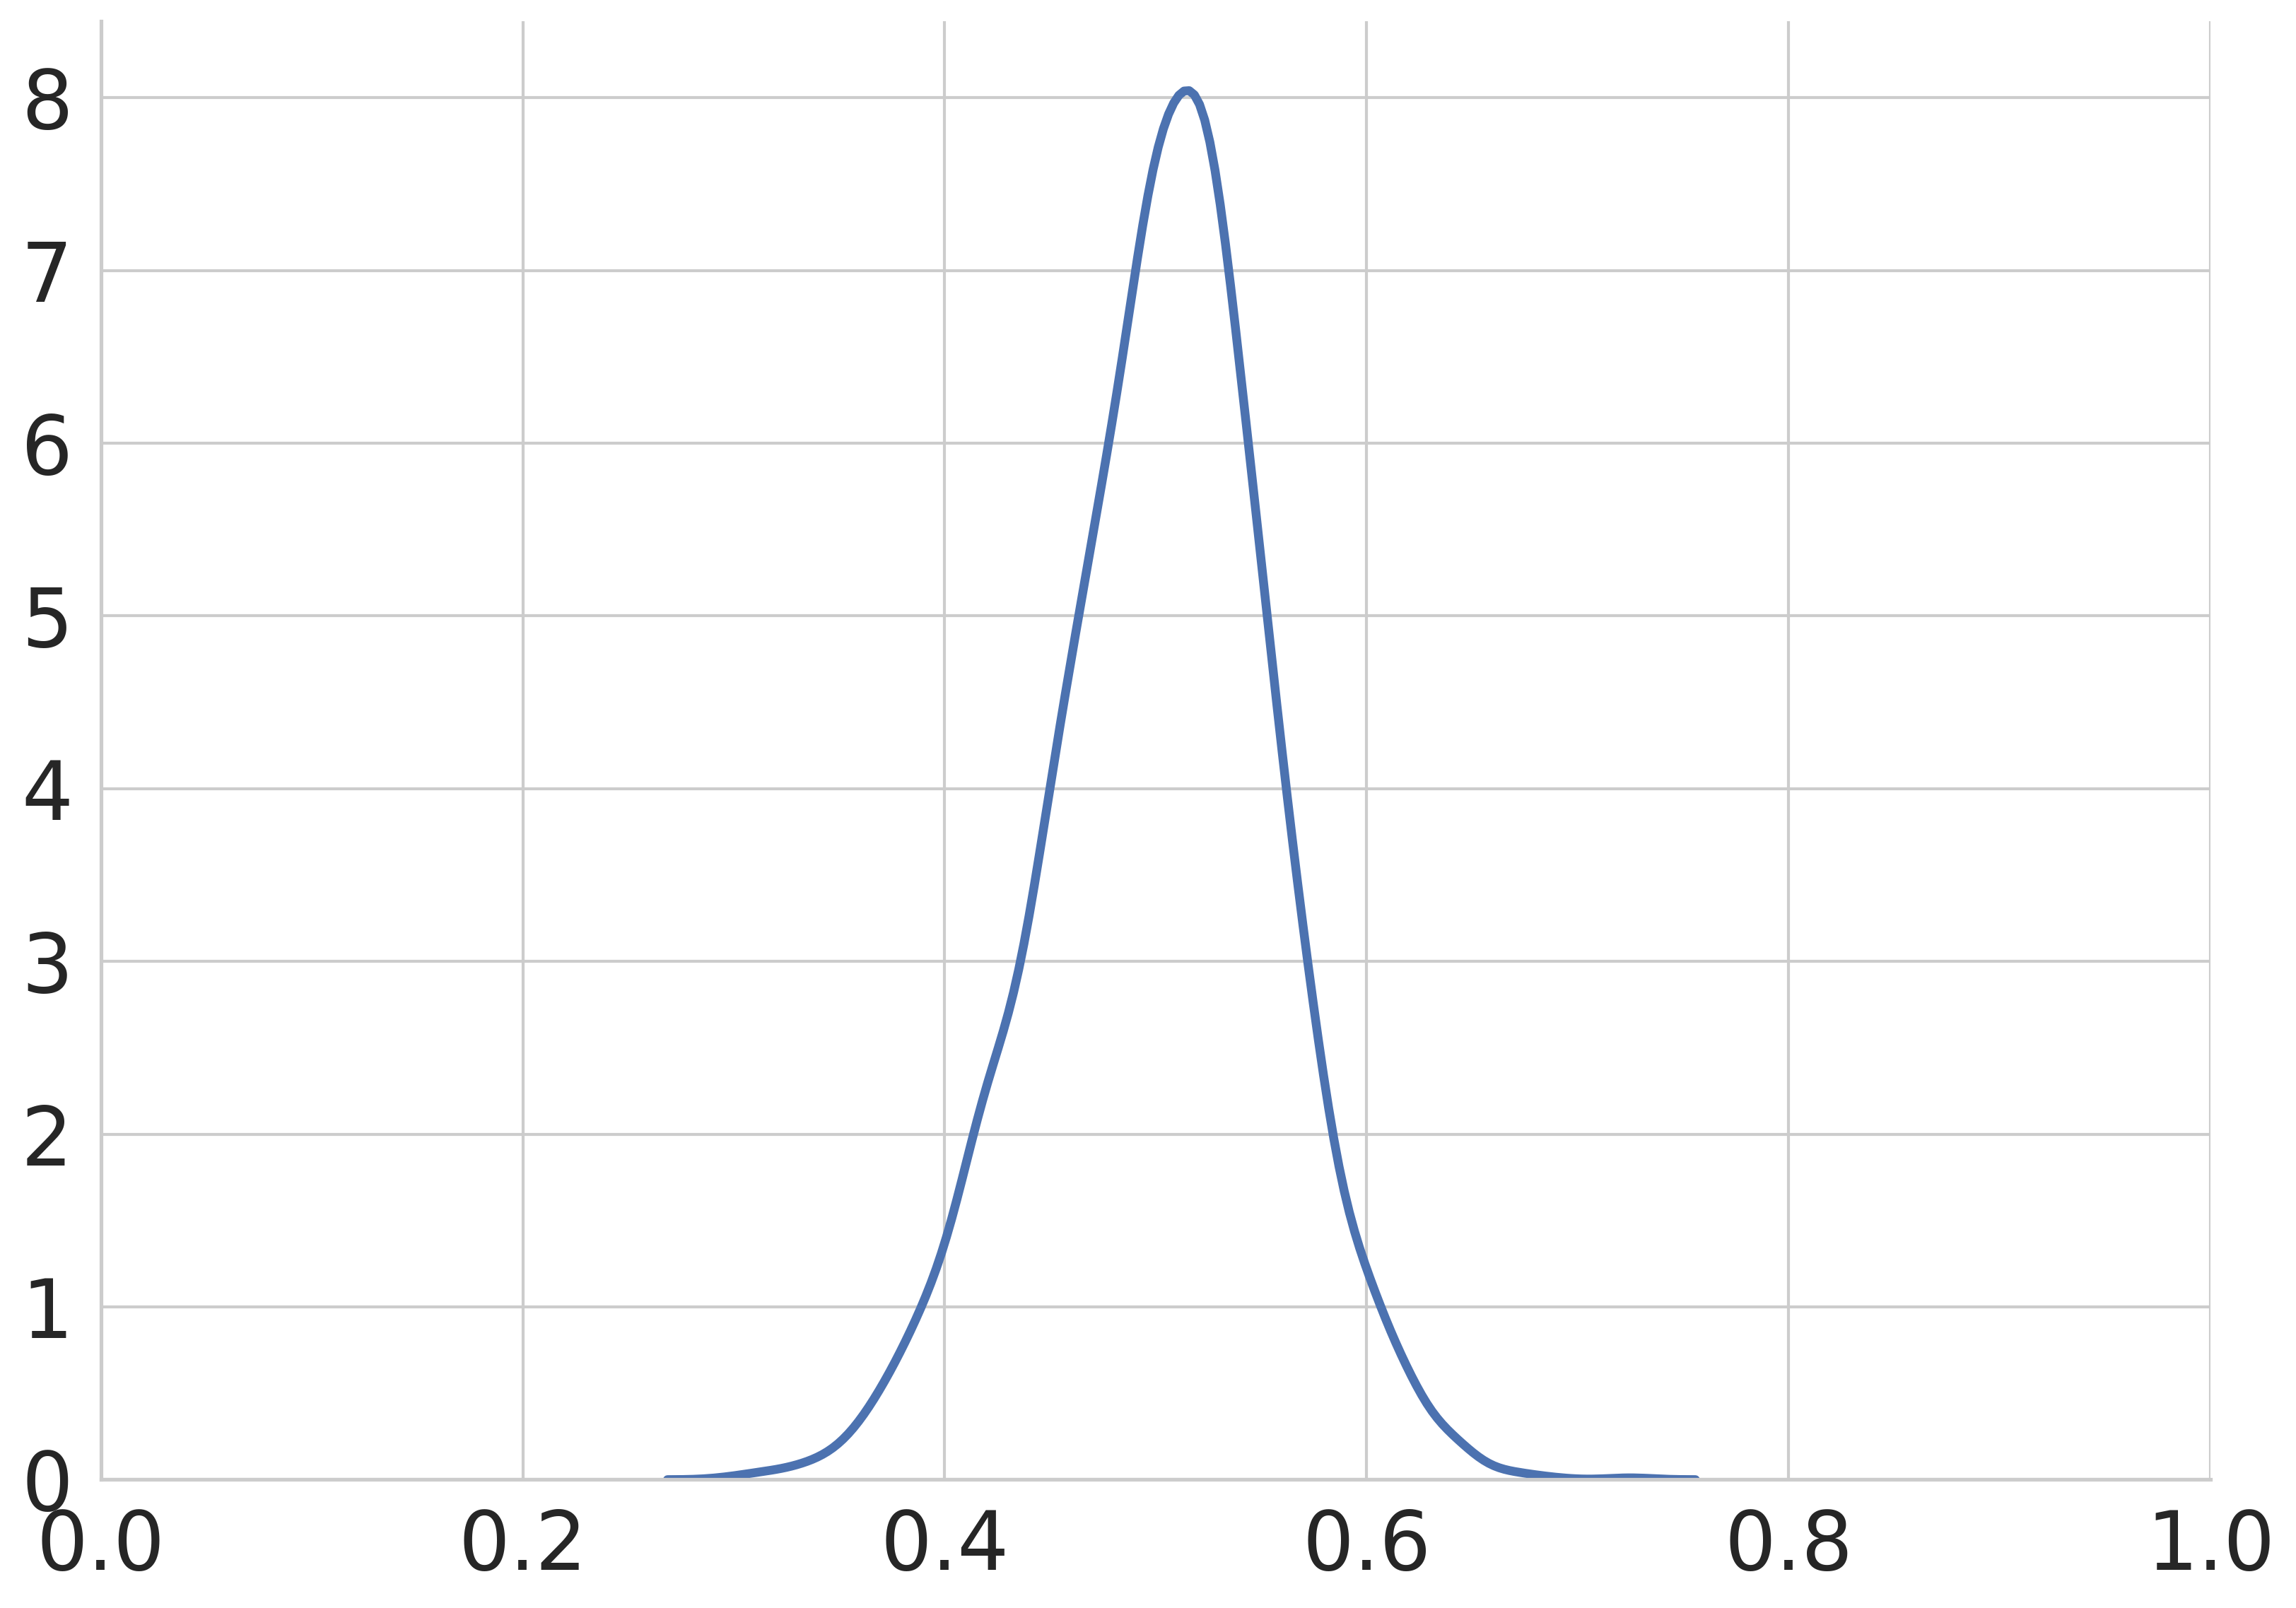
\includegraphics[scale=0.2]{figures/ps_photo_artpainting_temp10.png}
         \caption{Temperature scaling, with $\tau=10$.}
     \end{subfigure}
    \caption{
        Estimated propensity score distribution of \emph{photo} and \emph{art painting} on the
        PACS dataset. We compare (a) the original distribution ($\tau=1$) and (b) the
        temperature-scaled distribution ($\tau=10$). Here, the large temperature has the effect of
        transforming a bimodal distribution into a unimodal one.
}
    \label{fig:pacs_ps_pa}
\end{figure}
\begin{figure}[ht!]
     \centering
     \begin{subfigure}[b]{0.49\textwidth}
         \centering
         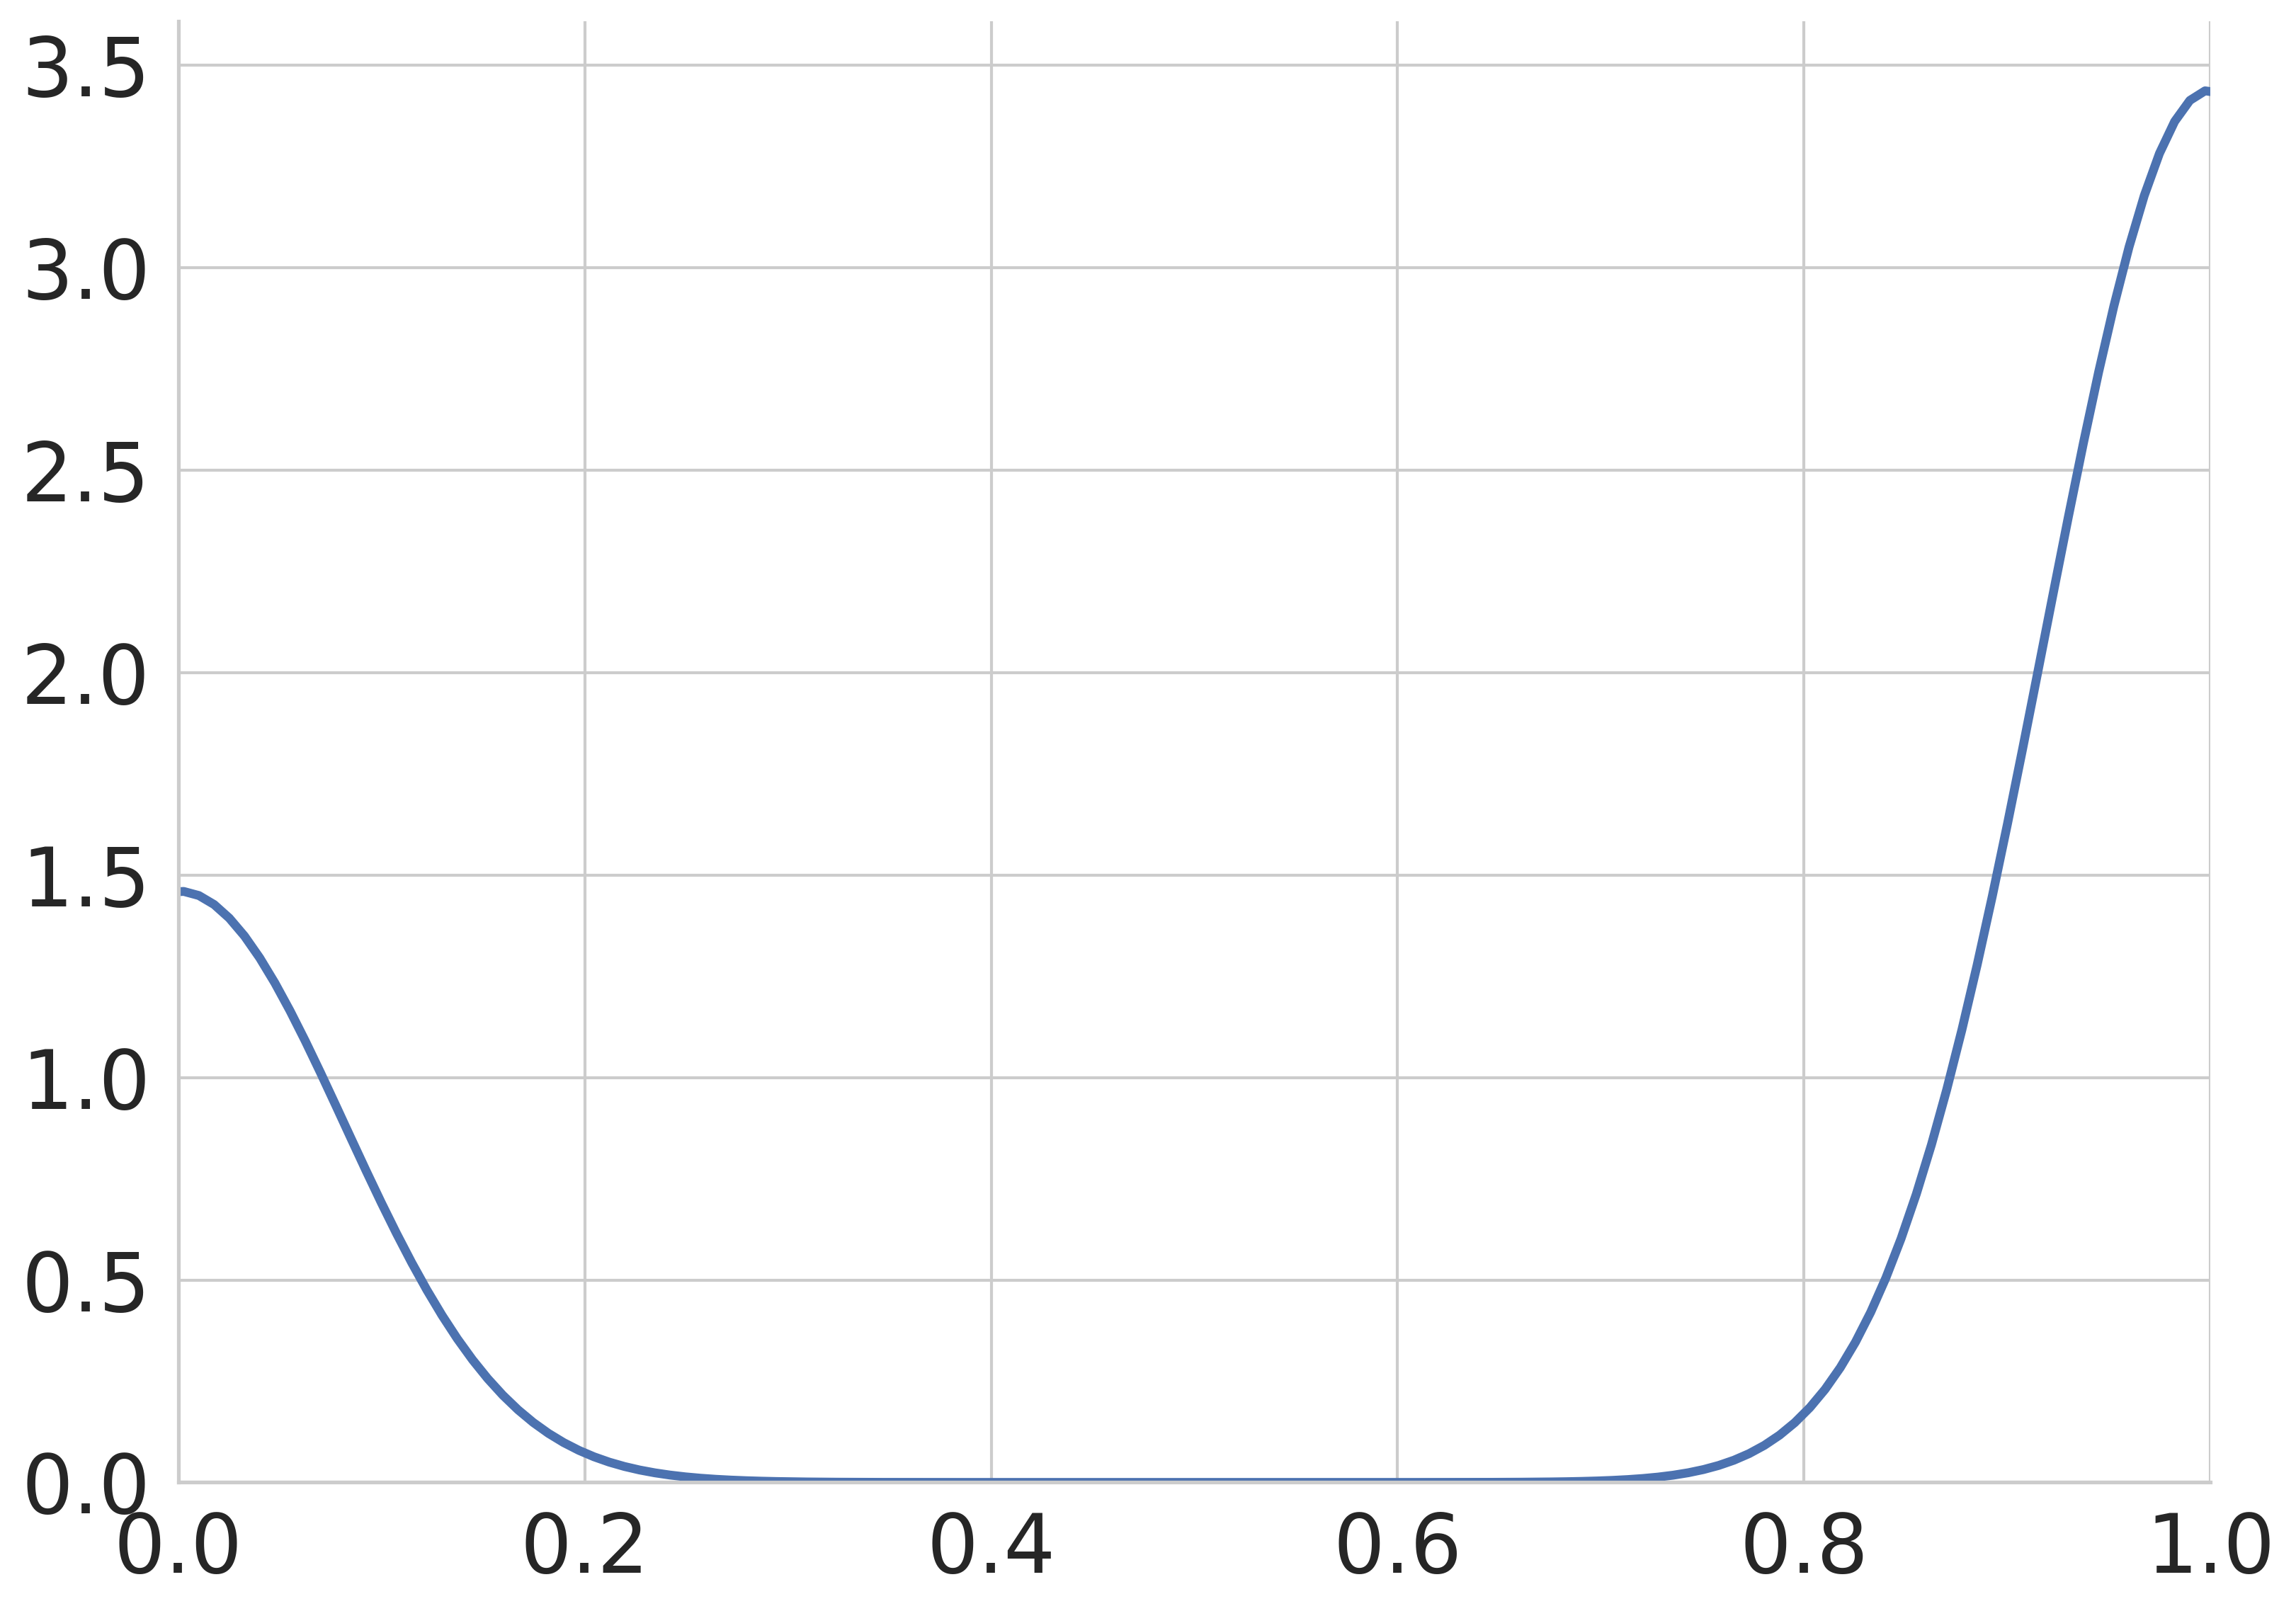
\includegraphics[scale=0.2]{figures/ps_photo_sketch_temp1.png}
         \caption{No temperature scaling ($\tau = 1$).}
     \end{subfigure}
     \hfill
     \begin{subfigure}[b]{0.49\textwidth}
         \centering
         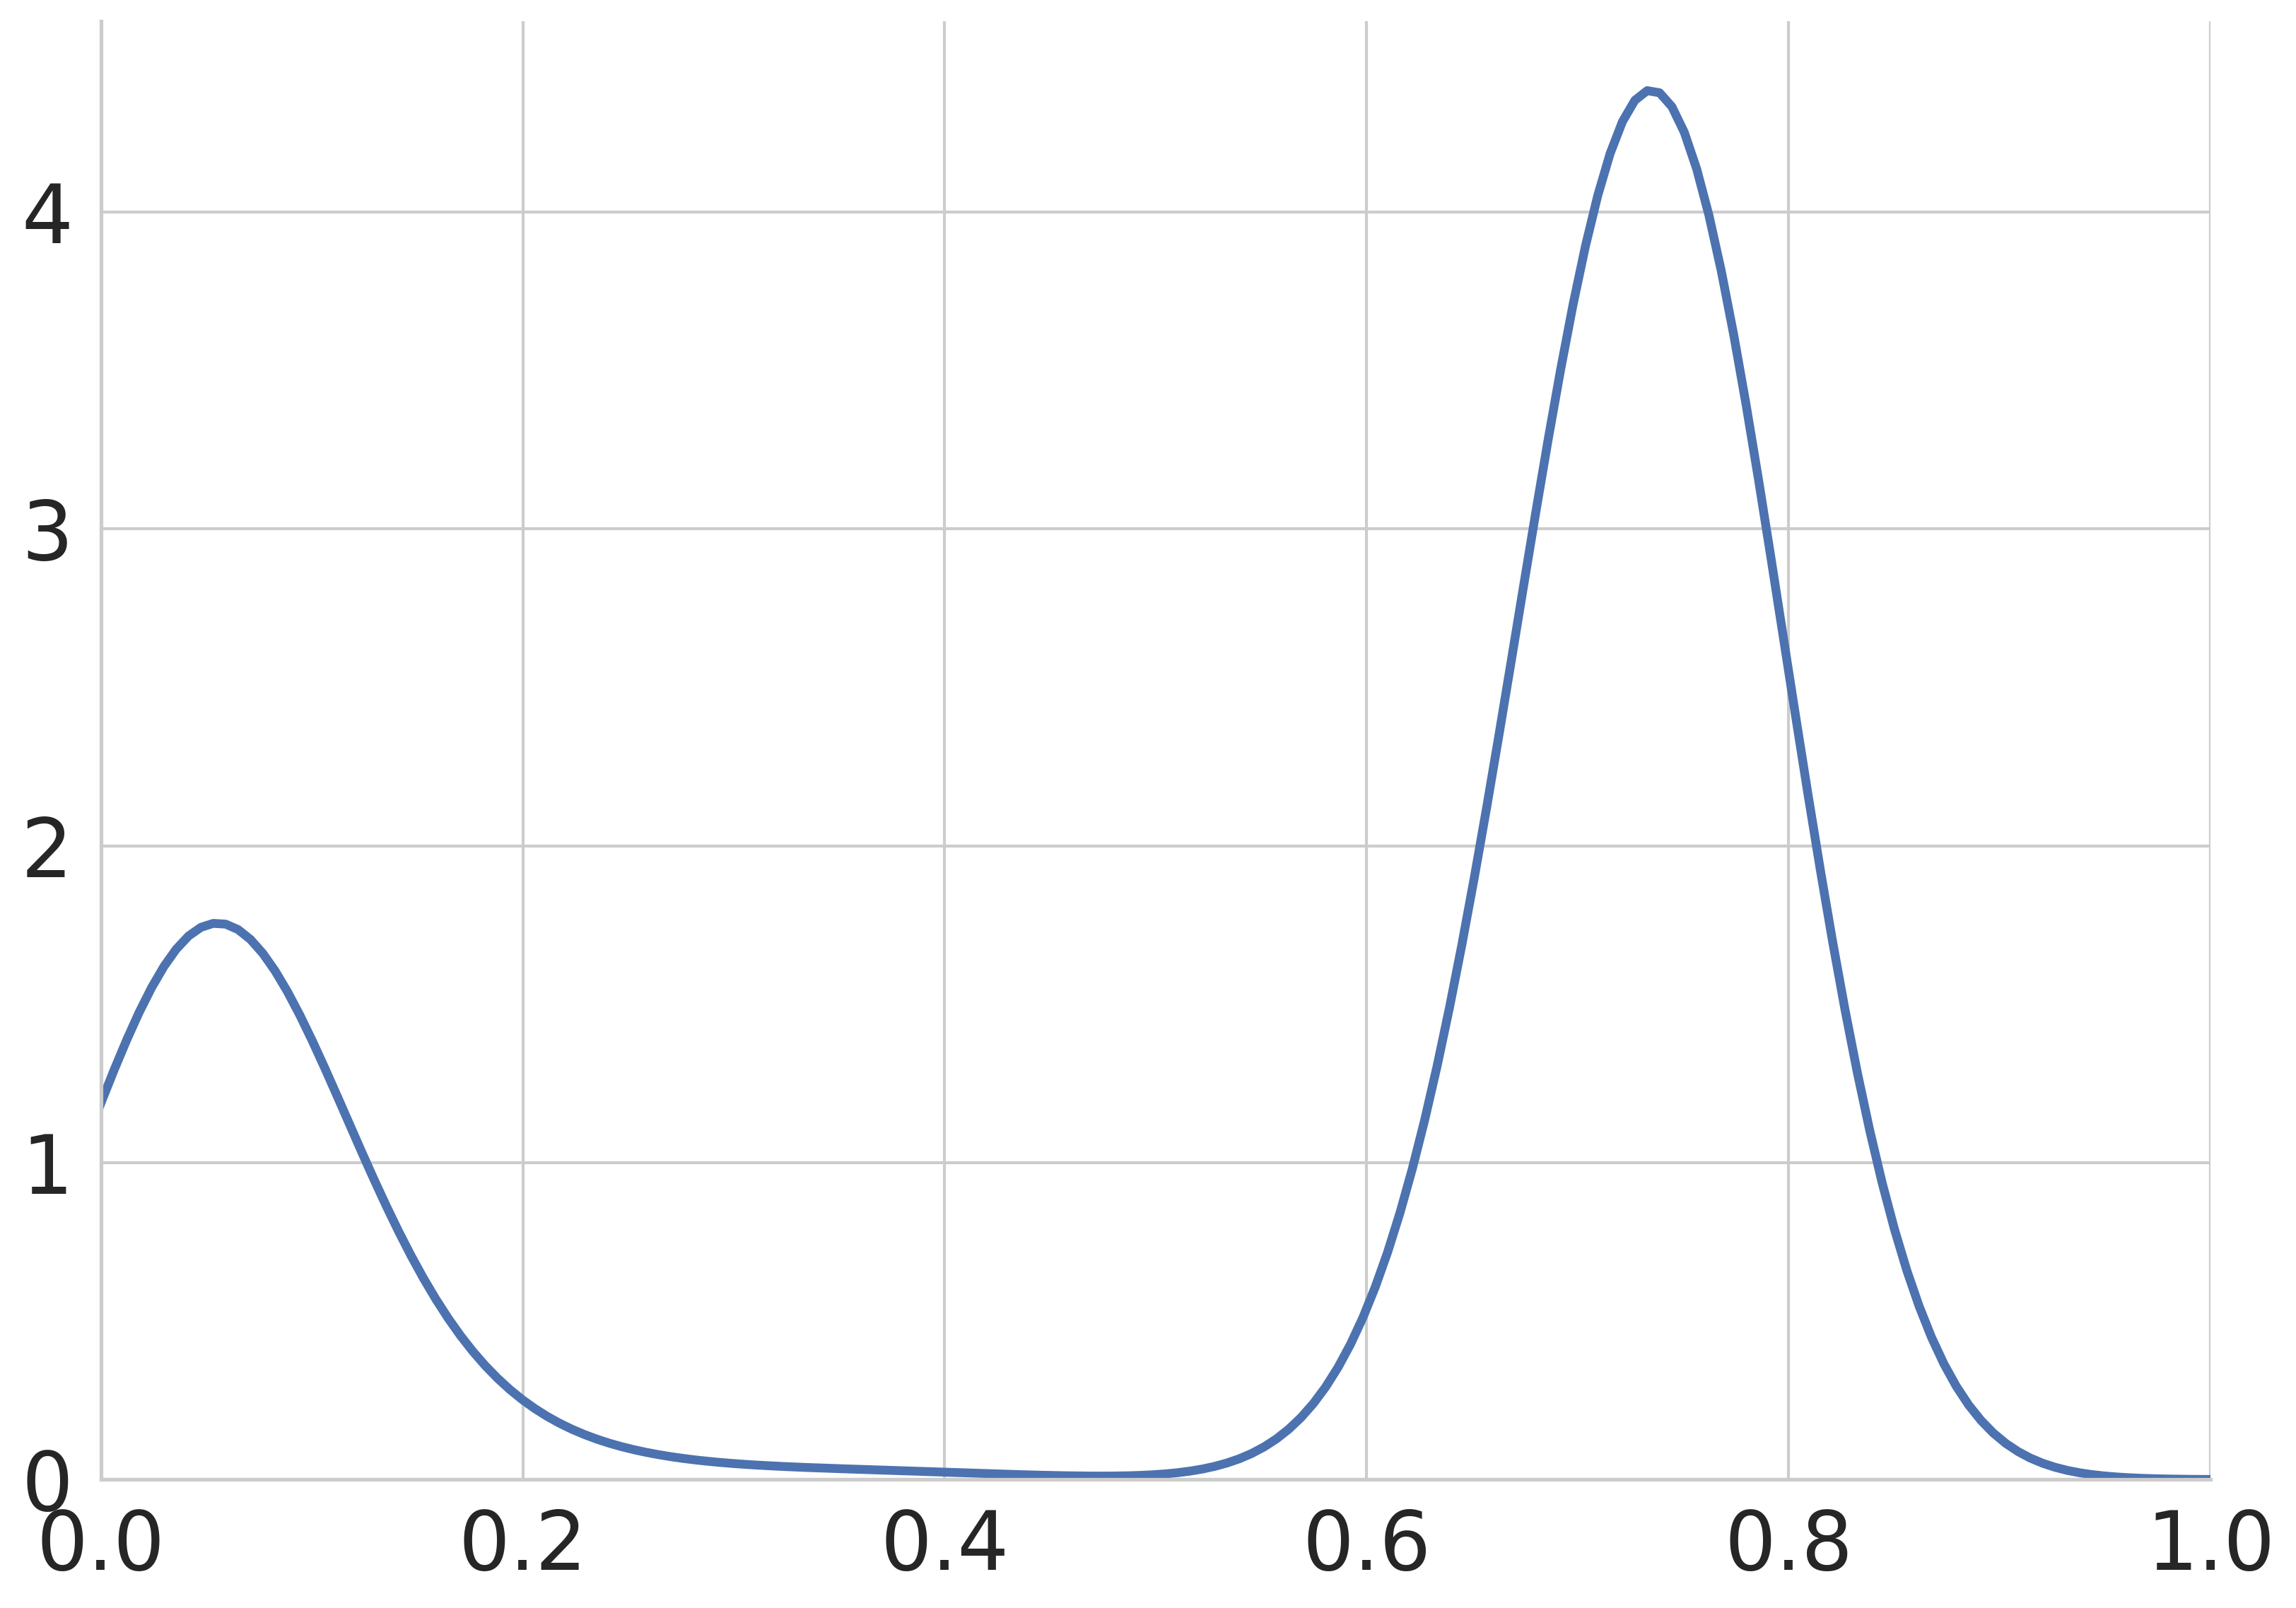
\includegraphics[scale=0.2]{figures/ps_photo_sketch_temp10.png}
         \caption{Temperature scaling, with $\tau=10$.}
     \end{subfigure}
    \caption{
        Estimated propensity score distribution of \emph{photo} and \emph{sketch} on the PACS
        dataset. We compare (a) the original distribution ($\tau=1$) and (b) the temperature-scaled
        distribution ($\tau=10$). Here, the large temperature has the effect of smoothing the
        distribution.
}
    \label{fig:pacs_ps_ps}
\end{figure}


\begin{table}[ht!]
	\centering
        \caption{
            Analysis of the number of the retrieved matched pairs when matching across the two
            domain \emph{photo} and \emph{sketch} on the PACS dataset. The fixed caliper
            threshold and temperature scaling can be used to smooth the propensity score
            distribution and effect the number of pairs.
}
	\scalebox{1.0}{
	\begin{tabular}{llll} 
	\toprule 
    \textbf{Fixed Caliper ($t_f$)}  & \textbf{Temperature ($\tau$)} & \textbf{photo} $\to$
    \textbf{sketch} & \textbf{sketch} $\to$ \textbf{photo} \\
    \midrule
    0.1 & 1 & 0 & 0 \\
    0 & 1 & 1540 & 3929 \\
    0.01 & 1 & 6 & 9 \\
    0.01 & 1.3 & 14 & 56 \\
    0.01 & 1.8 & 25 & 574 \\
    0.01 & 2.5 & 41 & 3082 \\
    0.01 & 10 & 1540 & 3929 \\
    0.1 & 10 & 298 & 3929 \\
	\bottomrule
	\end{tabular}}
	\label{tab:pacs_nsamples}
\end{table}


\begin{figure}[ht!]
  \centering
  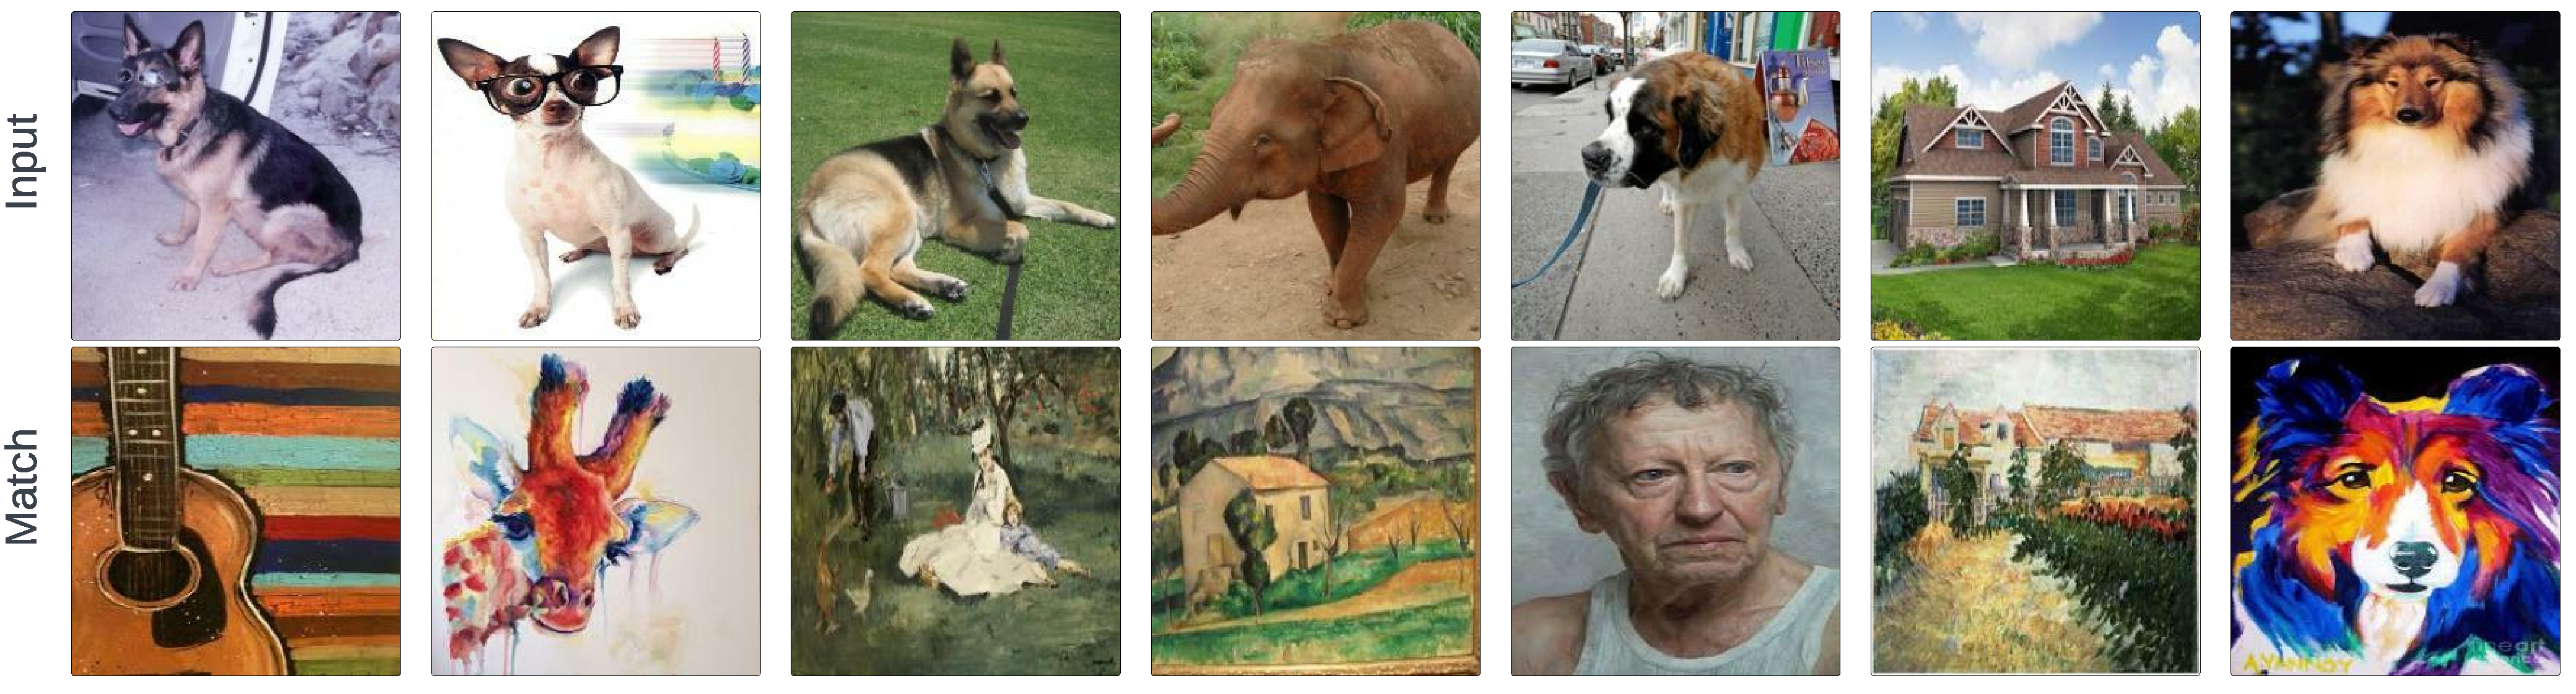
\includegraphics[width=1.\textwidth]{figures/matches_examples_pacs.pdf}
  \caption{
      Examples of input (photo) images and their 1-NN matched (art paint) images retrieved using
      \CNN{} from the PACS dataset. 
  %
  }
  \label{fig:match_pairs_pa}
\end{figure}
 
\begin{figure}[ht!]
  \centering
  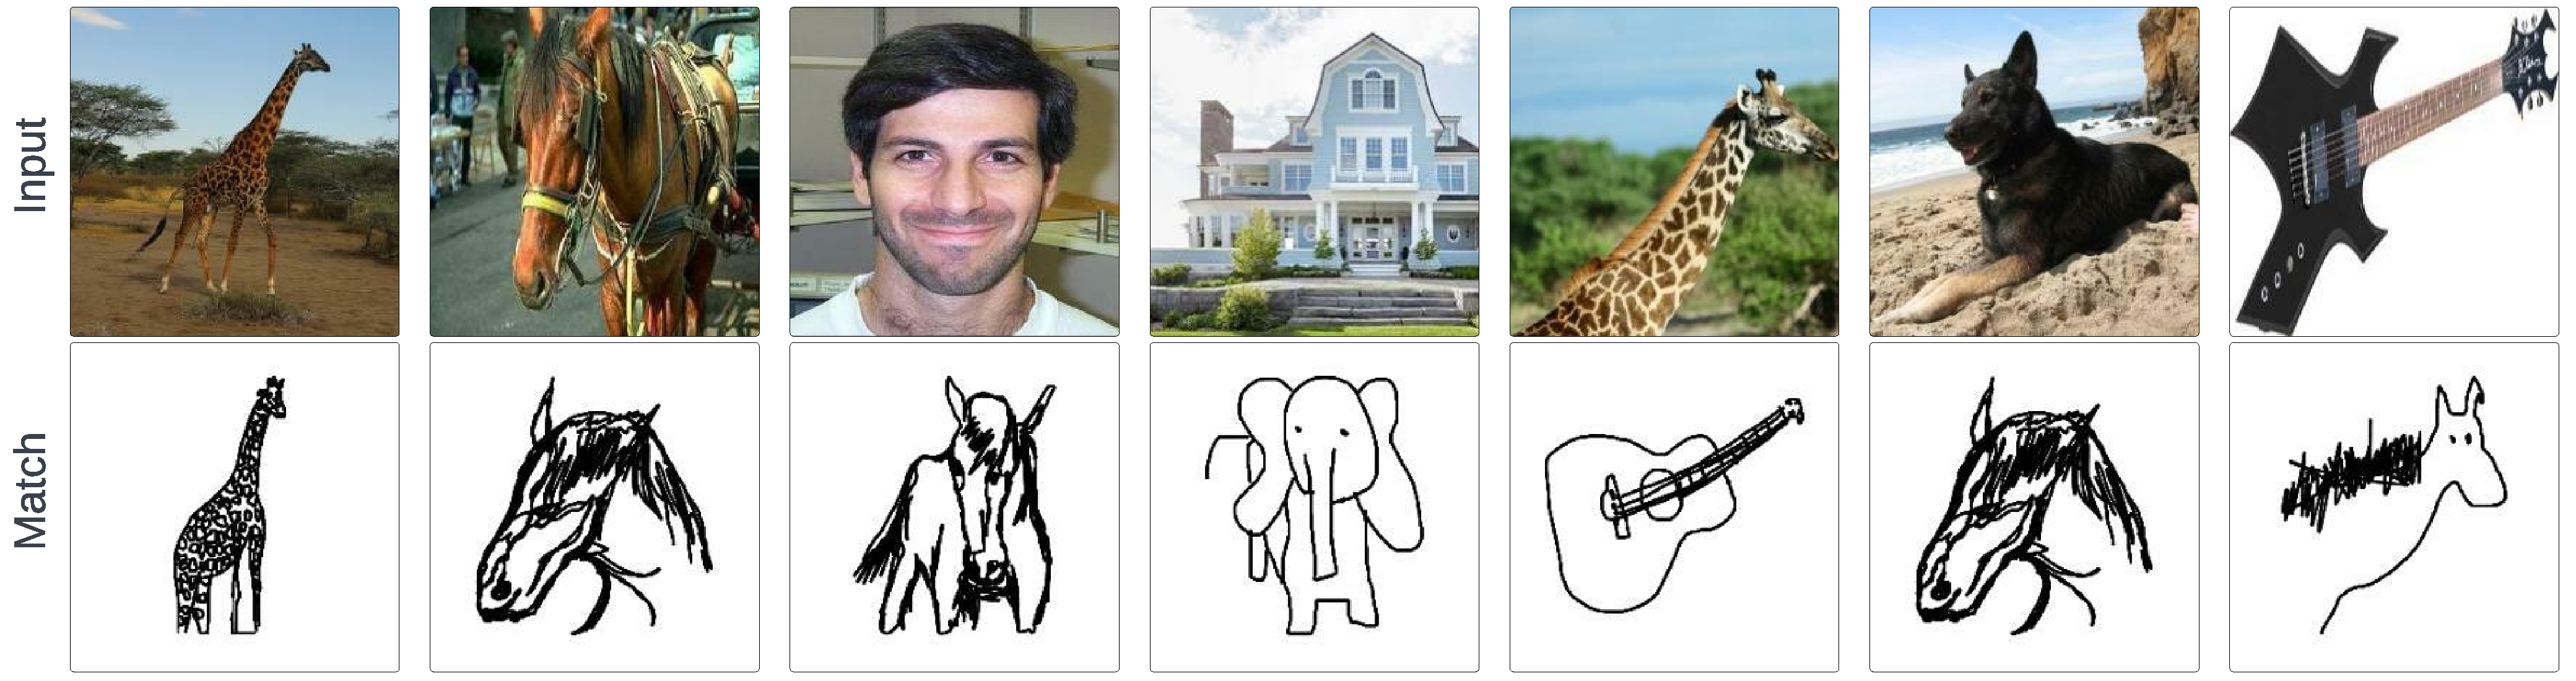
\includegraphics[width=1.\textwidth]{figures/matches_examples_pacs1.pdf}
  \caption{
      Examples of input (photo) images and their 1-NN matched (sketch) images retrieved using
      \CNN{}
      from the PACS dataset.
  %
  }
  \label{fig:match_pairs_ps}
\end{figure}


\subsection{Energy and Carbon Footprint Estimates}\label{appx:carbon}
\import{okapi}{carbon.tex}
